%%%%%%%%%%%%%%%%%%%%%%%%%%%%%%%%%%%%%%%%%%%%%%%%%%%%%%%%%%%%%%%%%%%%%%

\begin{figure}[]
	\begin{center}
	\scalebox{0.8}{
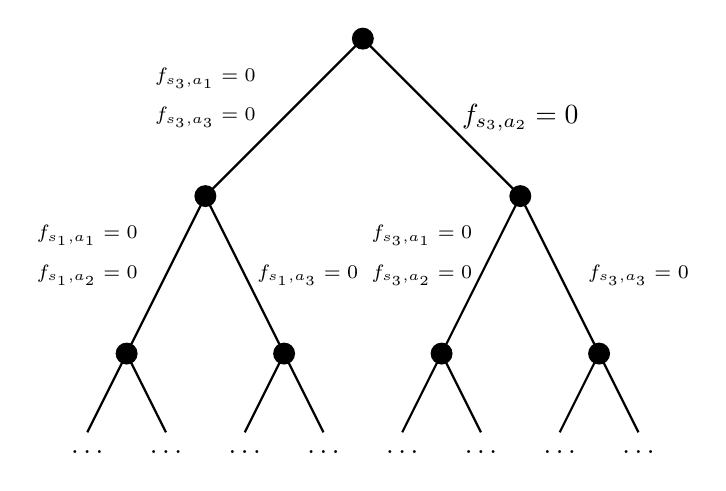
\begin{tikzpicture}

%da zero a 1
\draw[thick] (4,6) -- (2,4) ;
\node at (2,5.5) (Sentence) {{\scriptsize $f_{s_3,a_1}=0$}};
\node at (2,5) (Sentence) {{\scriptsize $f_{s_3,a_3}=0$}};


\draw[thick] (4,6) -- (6,4) ;
\node at (6,5) (Sentence) {{$\scriptsize f_{s_3,a_2}=0$}};


%da 1 a 2
\draw[thick] (2,4) -- (1,2) ;
\node at (0.5,3.5) (Sentence) {{\scriptsize $f_{s_1,a_1}=0$}};
\node at (0.5,3) (Sentence) {{\scriptsize $f_{s_1,a_2}=0$}};

\draw[thick] (2,4) -- (3,2) ;
\node at (3.3,3) (Sentence) {{\scriptsize $f_{s_1,a_3}=0$}};

\draw[thick] (6,4) -- (5,2) ;
\node at (4.75,3.5) (Sentence) {{\scriptsize $f_{s_3,a_1}=0$}};
\node at (4.75,3) (Sentence) {{\scriptsize  $f_{s_3,a_2}=0$}};


\draw[thick] (6,4) -- (7,2) ;
\node at (7.5,3) (Sentence) {{\scriptsize $f_{s_3,a_3}=0$}};

% da 2 in fondo
\draw[thick] (1,2) -- (0.5,1) ;
\node at (0.5,0.75) (Sentence) {$\dots$};

\draw[thick] (1,2) -- (1.5,1) ;
\node at (1.5,0.75) (Sentence) {$\dots$};

\draw[thick] (3,2) -- (2.5,1) ;
\node at (2.5,0.75) (Sentence) {$\dots$};

\draw[thick] (3,2) -- (3.5,1) ;
\node at (3.5,0.75) (Sentence) {$\dots$};

\draw[thick] (5,2) -- (4.5,1) ;
\node at (4.5,0.75) (Sentence) {$\dots$};

\draw[thick] (5,2) -- (5.5,1) ;
\node at (5.5,0.75) (Sentence) {$\dots$};

\draw[thick] (7,2) -- (6.5,1) ;
\node at (6.5,0.75) (Sentence) {$\dots$};

\draw[thick] (7,2) -- (7.5,1) ;
\node at (7.5,0.75) (Sentence) {$\dots$};


%livello 0
\draw[thick, fill =black] (4,6) circle (0.125);

%livello 1
\draw[thick, fill =black] (2,4) circle (0.125);%nodo radice
\draw[thick, fill =black] (6,4) circle (0.125);%nodo radice

%livello 2
\draw[thick, fill =black] (1,2) circle (0.125);%nodo radice
\draw[thick, fill =black] (3,2) circle (0.125);%nodo radice

\draw[thick, fill =black] (5,2) circle (0.125);%nodo radice
\draw[thick, fill =black] (7,2) circle (0.125);%nodo radice


\end{tikzpicture}
}
	\end{center}
\caption{Example of a branch-and-bound tree for an MDP with $4$ states and $3$ actions per state}
\label{fig:pic_bb}
\end{figure}
%%%%%%%%%%%%%%%%%%%%%%%%%%%%%%%%%%%%%%%%%%%%%%%%%%%%%%%%%%%%%%%%%%%%%
